\documentclass[10pt,a4paper]{article}
\usepackage[utf8]{inputenc}
\usepackage[italian]{babel}
\usepackage{amsmath}
\usepackage{amsfonts}
\usepackage{amssymb}
\usepackage{graphicx}
\usepackage[left=2cm,right=2cm,top=2cm,bottom=2cm]{geometry}
\newcommand{\rem}[1]{[\emph{#1}]}
\newcommand{\exn}{\phantom{xxx}}

\author{Gruppo 1G.BT \\ Lorenzo Cavuoti, Francesco Sacco}
\title{Es01B: Misure di tensione, corrente, tempi, frequenza.}
\begin{document}
\date{4 Ottobre 2018}
\maketitle

\setcounter{section}{1}
\section{Misure di tensione e corrente}

\paragraph{2.b Partitore con resistenze da circa 1~k}
Valori misurati $R_1$ e $R_2$ e valore atteso di $A_\mathrm{exp}$:
\[
R_1 = (1182 \pm 9) \,\mathrm{k}\Omega, \quad
R_2 = (971 \pm 7) \,\mathrm{k}\Omega, \quad
A_\mathrm{exp} = ( 0.452 \pm 0.004 ) 
\]


\begin{table}[h]
\centering
\begin{tabular}{|c|c|c|c|c|c|}
\hline 
VIN& $\sigma$ VIN  &VOUT	 & $\sigma$ VOUT& VOUT/VIN & $\sigma$ VOUT/VIN \\
\hline 
1,928 & 0,009 & 0,868 & 0,004 & 0.450 &\exn 0.005 \\
5,94 & 0,03 & 2,68 & 0,02 & 0.451 &\exn 0.005 \\
4,24 & 0,02 & 1,91 & 0,01 & 0.450 &\exn 0.005 \\
2,65 & 0,02 & 1,194 & 0,006 & 0.451 &\exn 0.005 \\
6,19 & 0,17 & 2,80 & 0,02 & 0.452 &\exn 0.005 \\
7,28 & 0,03 & 3,29 & 0,02 & 0.452 &\exn 0.005 \\
8,41 & 0,04 & 3,80 & 0,02 & 0.452 &\exn 0.005 \\
9,79 & 0,04 & 4,42 & 0,02 & 0.451 &\exn 0.005 \\
0,868 & 0,004 & 0,392 & 0,002 & 0.452 &\exn 0.005 \\
\hline 
\end{tabular} 
\caption{(2.b) Partitore di tensione con resistenze da circa 1k. Tutte le tensioni in V.\label{t:par1}}
\end{table}

\begin{figure}[h]
\centering
%\includegraphics[scale=0.4]{part1.pdf}
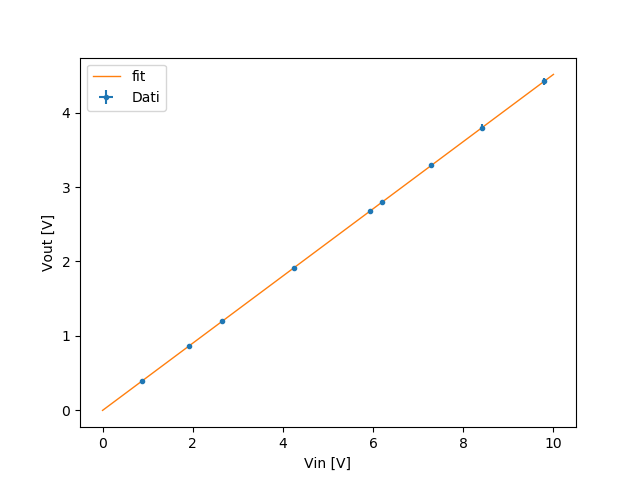
\includegraphics[scale=0.6]{plot_2b.png}
 

\caption{(2.b) Grafico $V_{out}$ vs. $V_{in}$ con resistenze di circa 1k \label{f:par1}}
\end{figure}

\framebox(400,30){Inserire commento sul confronto tra valori misurati ed attesi.}


\paragraph{2.c Partitore con resistenze da circa 4M}
Valori misurati $R_1$ e $R_2$ e valore atteso di $A_\mathrm{exp}$:
\[
R_1 = ( 3,80 \pm 0,04 ) \,\mathrm{M}\Omega, \quad
R_2 = ( 4,81 \pm 0,05 ) \,\mathrm{M}\Omega, \quad
A_\mathrm{exp} = ( 0.559 \pm 0.005 ) 
\]


\begin{table}[h]
\centering
\begin{tabular}{|c|c|c|c|c|c|}
\hline 
VIN& $\sigma$ VIN  &VOUT	 & $\sigma$ VOUT& VOUT/VIN & $\sigma$ VOUT/VIN \\
\hline 
0,754 & 0,003 & 0,347 & 0,002 & 0.460 & 0.005 \\
1,825 & 0,009 & 0,839 & 0,004 & 0.460 & 0.005 \\
2,89 & 0,02 & 1,332 & 0,007 & 0.461 & 0.005\\
4,150 & 0,02 & 1,910 & 0,010 & 0.460 & 0.005\\
5,26 & 0,03 & 2,42 & 0,01 & 0.460 & 0.005\\
7,02 & 0,04 & 3,24 & 0,02 & 0.461 & 0.005\\
8,13 & 0,04 & 3,74 & 0,02 & 0.460 & 0.005\\
9,23 & 0,05 & 4,25 & 0,02 & 0.460 & 0.005\\
6,17 & 0,03 & 2,48 & 0,02 & 0.460 & 0.005\\
\hline 
\end{tabular} 
\caption{(2.c) Partitore di tensione con resistenze da circa 4M. Tutte le tensioni in V.\label{t:par2}}
\end{table}


\begin{figure}[h]
\centering
%\includegraphics[scale=0.4]{part1.pdf}
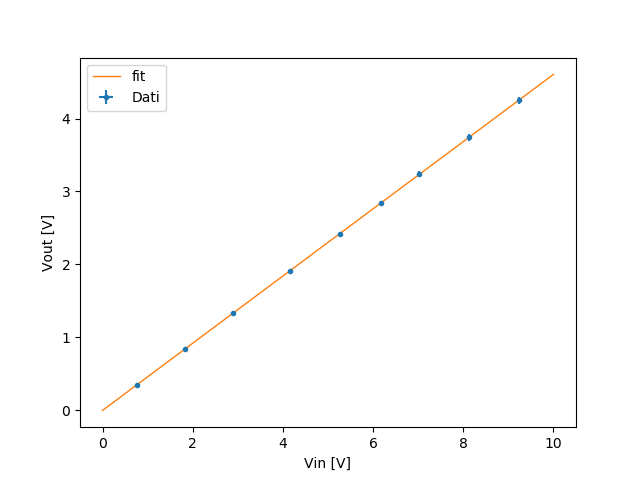
\includegraphics[scale=0.6]{plot_2c.png}

\caption{(2.c) Grafico $V_{out}$ vs. $V_{in}$ con resistenze da circa 4M \label{f:par2}}
\end{figure}

\framebox(400,30){Inserire commento sul confronto tra valori misurati ed attesi.}



\paragraph{2.d Resistenza di ingresso del tester}
Usando il modello mostrato nella scheda si ottiene
\[ \frac{R_1}{R_T} =  \frac{V_{IN}}{V_{OUT}} - (1 +  \frac{R_1}{R_2} )
\]

Con i dati del punto 2.b si ottiene
\[ R_1/R_T = \exn  \pm  \exn   \rightarrow  R_1 > \exn k\Omega
\]


Con i dati del punto 2.c si ottiene
\[ R_1/R_T = \exn  \pm  \exn   \rightarrow  R_1 = (\exn \pm  \exn)  M\Omega
\]


\framebox(400,30){Inserire commento sulla sensibilit\`a sperimentale della misura.} 


\section{Uso dell'oscilloscopio}

\paragraph{3.b Misure di tensione} 
Vengono ripetute le misure del punto 2.c  ma con pochi punti e senza grafico
\begin{table}[h]
\centering
\begin{tabular}{|c|c|c|c|c|c|}
\hline 
VIN& $\sigma$ VIN  &VOUT	 & $\sigma$ VOUT& VOUT/VIN & $\sigma$ VOUT/VIN \\
\hline 
1,76 & 0,07 & 0,776 & 0,031 & 0.44 & 0.03\\
4,64 & 0,18 & 2,12 & 0,08 & 0.46 & 0.04 \\
7,6 & 0,3 & 3,32 & 0,13 & 0.44 & 0.03 \\
9,8 & 0,4 & 4,40 & 0,17 & 0.45 & 0.04 \\
\hline 
\end{tabular} 
\caption{(3.b) Partitore di tensione con resistenze da circa 4M, misura con oscilloscopio. Tutte le tensioni in V.}
\end{table}


\paragraph{3.d Impedenza di ingresso dell'oscilloscopio} Si ripete l'analisi del punto 2.d

\[ R_1/R_{IN} = \exn  \pm  \exn   \rightarrow  R_{IN} = (\exn \pm  \exn)  M\Omega
\]


\section{Misure di frequenza e tempo}

\paragraph{4.b Misure di frequenza}
Misure con onda sinusoidale
\begin{table}[h]
\centering
\begin{tabular}{|c|c|c|c|c|c|}
\hline 
Periodo T (s)& $\sigma$ T (s)  &Frequenza f (Hz) & $\sigma$ f (Hz) & Misura oscilloscopio (Hz) & Differenza (Hz)\\
\hline 
1,01 \times 10^{-3} & 0,01 \times 10^{-3} & 997 & 10 & 997 &7 \\
1,02 \times 10^{-4} & 0,01 \times 10^{-4}& 9,8 \times 10^3 & 0,1 \times 10^3 & 9,9\times10^3 &10^2 \\
1,00 \times 10^{-5} &0,01 \times 10^{-5}& 1,0 \times 10^5 & 0,01 \times 10^5  & 9,99\times10^3 &10^2\\
1,01 \times 10^{-6} &0,01 \times 10^{-6}& 9,90 \times 10^5 & 0,01 \times 10^5 & 1,00\times 10^6 &1,4\times10^4 \\
\hline 
\end{tabular} 
\caption{(4.b) Misura di frequenza di onde sinusoidali  e confronto con misurazione interna dell'oscilloscopio }
\end{table}



\section{Trigger dell'oscilloscopio}
\paragraph{5.b Segnale pulse}
Misure con segnale pulse del generatore di onde
\begin{figure}[h]
\centering
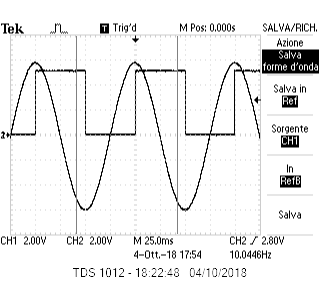
\includegraphics[scale=0.9]{screen_osc.png}
\caption{(5.b) Relazione temporale tra il segnale pulse e l'onda principale}
\end{figure}


\section{Conclusioni e commenti finali}
\framebox(400,30){Inserire eventuali commenti e conclusioni finali}

\section*{Dichiarazione}
I firmatari di questa relazione dichiarano che il contenuto della relazione \`e originale, con misure effettuate dai membri del gruppo, e che tutti i firmatari hanno contribuito alla elaborazione della relazione stessa.

\end{document}
